\documentclass[11pt]{article}
\usepackage{graphicx}

\usepackage[backend=biber,style=numeric, sorting=none]{biblatex}
\addbibresource{bibliografia.bib}
\defbibheading{bibliography}[\textbf{RIFERIMENTI BIBLIOGRAFICI}]{%
\begin{center}
    \textbf{\large #1}  % Titolo centrato e in grassetto (puoi cambiare \Large se vuoi)
\end{center}}

\usepackage{amsmath, esint,amsthm,amssymb,graphicx,mathtools,tikz,hyperref,multicol,cancel,enumitem,booktabs,float,pgfplots,multirow,mathrsfs,textcomp,gensymb,soul,changepage,threeparttable}
\renewcommand{\CancelColor}{\color{rosso}}

\usepackage[a4paper, margin=2cm]{geometry}
\usepackage{tabularx}
\usepackage{titlesec}
\usepackage[italian]{babel}
\usepackage{float}
\usepackage{fontspec}
\usepackage{setspace}
\usepackage{caption}

\setmainfont{calibri.ttf}[Path=./fonts/,Extension=.ttf,BoldFont=calibri_bold.ttf,ItalicFont=calibri_italic.ttf]

\setlength{\parskip}{0pt}

\DeclareCaptionLabelFormat{customformat}{{\textbf{#1~#2}}}
\captionsetup{
    font={small, it},
    labelformat=customformat,
    labelsep=colon,
    justification=raggedright,
    singlelinecheck=true
}

\begin{document}

% \maketitle
\begin{center}
    {\textbf{\Large Laboratorio di Elettromagnetismo e Ottica}}\\[0.5cm]
    {\textbf{\Large Prova 3: Misura di Resistenze e Ponte di Wheatstone}}\\[0.7cm]
    {\large Emanuele Martelli \\ Davide Rizzi \\ David Santiago Caballero \\ Simone Zucchi}\\[0.7cm]
    {\large 10 dicembre 2025}
\end{center}

\section{Risultati e discussione}
In questa sezione verranno riportati i dati raccolti e la relativa analisi statistica che ne ha permesso la determinazione delle incertezze.
\subsection{DMM}

\begin{table}[h]
\centering
\begin{tabular}{|c|c|c|}
\hline
\textbf{Grandezza} &
\textbf{Valore $(\Omega)$} &
\textbf{Incertezza $(\Omega)$} \\
\hline
$R_1$ & 15.57 & 0.04 \\ \hline
$R_2$ & 679.87 & 0.40 \\ \hline
$R_3$ & 14911 & 17 \\ \hline
$R_1 + R_2$ & 694.5 & 0.4 \\ \hline
$R_1 / R_2$ & 14.896 & 0.04 \\ \hline
$R_{min}$ & 0.426 & 0.03 \\ \hline
$R_{max}$ & 994.0 & 1.4 \\ \hline
\end{tabular}
\caption{\textit{Tabella dei valori delle resistenze mirurati mediante multimetro digitale della scheda Elvis con rispettive incertezze. Nelle ultime 2 righe si riporta il valore minimo e massimo di resistenza del potenziometro.}}
\label{tab:resistenze}
\end{table}

La misura delle resistenze, effettuata con il multimetro della scheda Elvis, ha prodotto i risultati sopra riportati (Tabella 1). Le incertezze, di natura strumentale, sono state stimate a partire dalle specifiche della scheda stessa. L'incertezza sulla resistenza è stata misurata come $\pm (\text{ppm of reading} + \text{ppm of of range})$ dove:
\begin{itemize}
    \item reading: valore della resistenza misurato dal multimetro digitale.
    \item range: scegliere il più opportuno tra i valori di resistenza proposti nella tabella. Il range scelto deve essere maggiore del valore della resistenza incognita.
\end{itemize}

% \begin{figure}[H]
%     \centering
%     \includegraphics[width=1.0\linewidth]{delta_r.png}
%     \caption{\textit{Riga della tabella per il calcolo delle incertezze della resisteza presa dal manuale della scheda Elvis}}
%     \label{fig:placeholder}
% \end{figure}

Supponiamo di voler calcolare l'incertezza associata alla misura della resistenza da $15 \Omega$. In questo caso scegliamo il range di $100 \Omega$, ne consegue che $$\Delta\Omega = (450\cdot\frac{\text{reading}}{10^6} +310\cdot\frac{\text{range}}{10^6})$$.

Ci siamo inoltre assicurati che le incertezze così calcolate sulla serie e sul parallelo fossero comparabili con quelle ricavate mediante propagazione lineare degli errori.

I valori misurati sono dell'ordine di grandezza corretto ma non risultano compatibili con quelli attesi. La causa di ciò è da ricercare proprio nel valore nominale delle resistenze; quest'ultimo infatti non è altro che un riferimento al quale, il costruttore, associa una tolleranza (nel nostro caso del 5\%).
Tenendo conto di ciò i dati raccolti risultano coerenti e compatibili con quanto atteso.


\subsection{Legge di Ohm}

\begin{table}[H]
\centering
\begin{tabularx}{\textwidth}{|c|c|c|X|X|}
\hline
\textbf{Grandezza} &
\textbf{Valore $(\Omega)$} &
\textbf{Incertezza $(\Omega)$} &
\textbf{Valore (py program) $(\Omega)$} &
\textbf{Incertezza (py program) $(\Omega)$} \\
\hline
$R_1$ & 15.0111 & 0.0244 & 15.04 & 0.02 \\ \hline
$R_2$ & 679.688 & 0.4526 & 679.66 & 0.23 \\ \hline
$R_3$ & 15118.2 & 168.34 & 15127.59 & 86.88 \\ \hline
$R_1 + R_2$ & 694.646 & 0.362106 & 694.33 & 0.17 \\ \hline
$R_1 / R_2$ & 14.7315 & 0.0297885 & 14.73 & 0.01 \\ \hline
\end{tabularx}
\caption{Tabella dei valori delle resistenza con le rispettive incertezze. Le prime due colonne riportano l'output del programma di analisi dati scritto in LabView utilizzato durante la presa dati. Le ultime due colonne riportano le stesse grandezze ma ricavate mediante fit lineare effettuato in python.}
\label{tab:resistenze}
\end{table}

La misura delle resistenze mediante applicazione della legge di Ohm ha prodotto i risultati sopra riportati (Tabella 2).
Il programma di acquisizione dati in LabView ha permesso di calcolare la resistenza mediante regressione lineare dei punti nel piano tensione(V) - corrente(I). La resistenza corrisponde infatti al reciproco del coefficiente angolare della retta del fit.
Abbiamo rianalizzato i dati eseguendo un fit in python e ne abbiamo riportato i risultati nelle ultime due colonne (Tabella 2).

\begin{figure}[H]
    \centering
    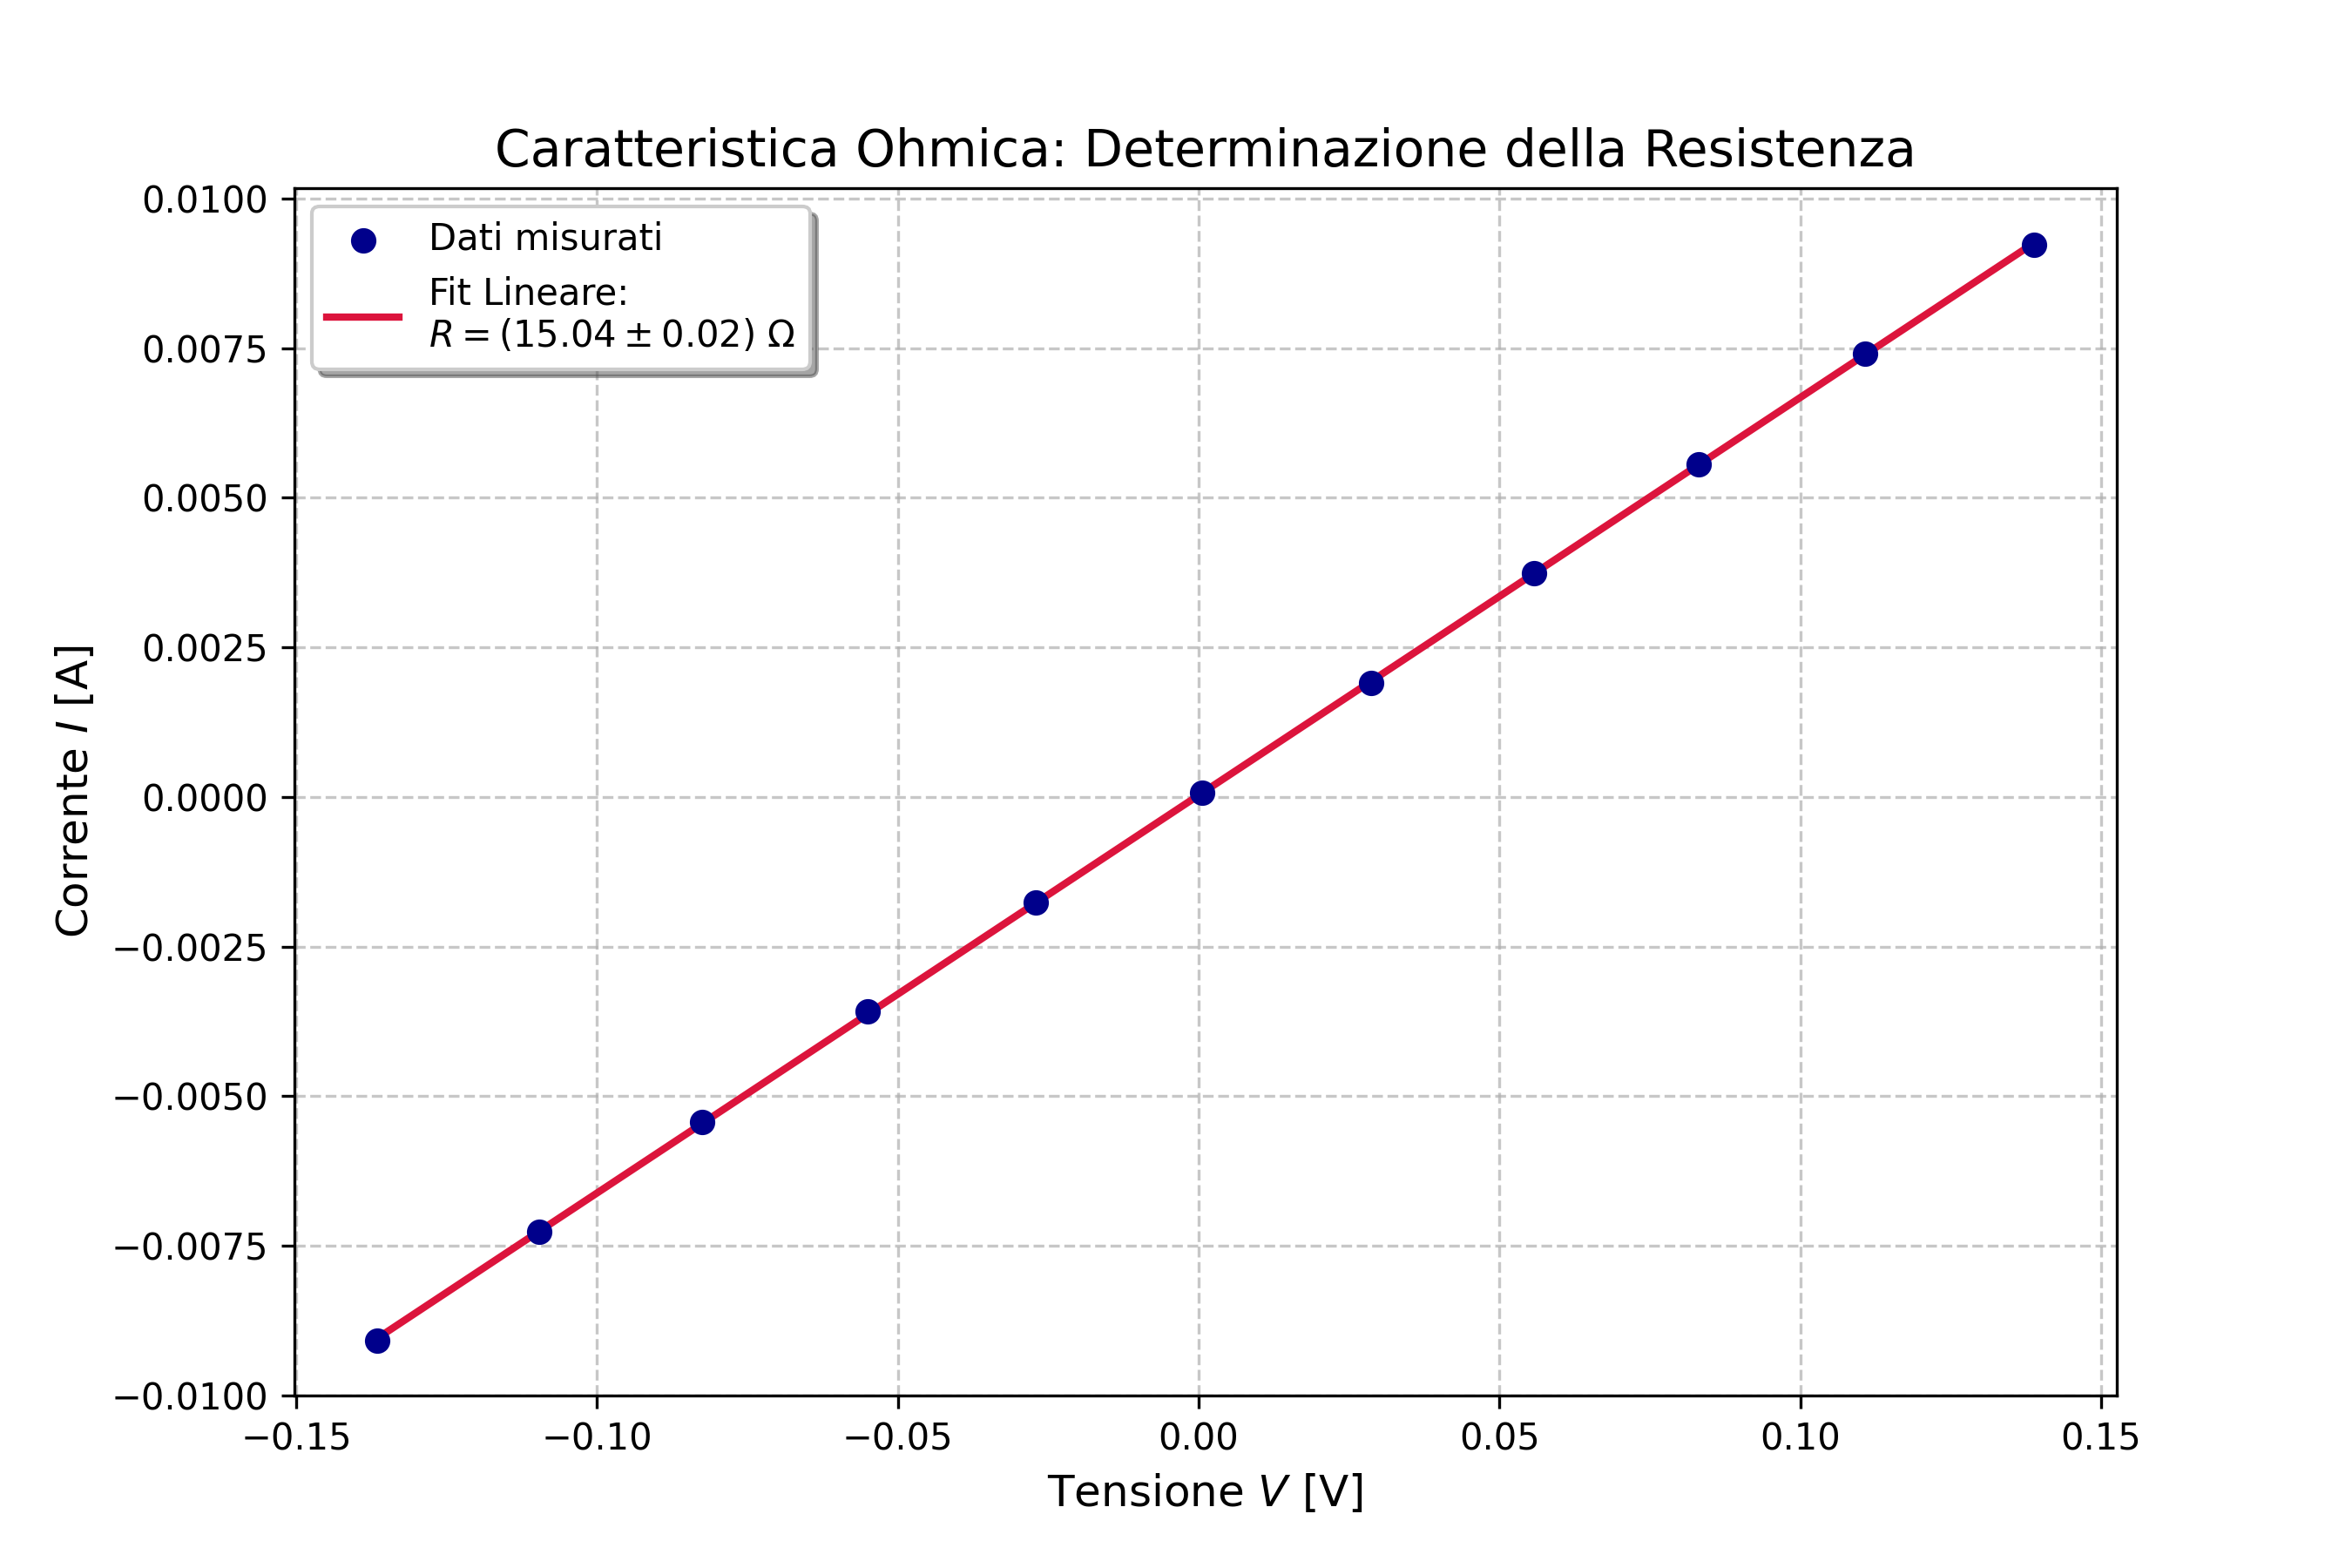
\includegraphics[width=1.0\linewidth]{figures/Grafico_Ohm_Incertezza.png}
    \caption{Grafico Tensione-Corrente e fit lineare ricavato mediante numpy.polyfit.}
    \label{fig:placeholder}
\end{figure}

Durante la presa dati, si è osservato che, per la resistenza da $15\Omega$, per via del setup sperimentale, non era possibile effettuare la presa dati per tensioni superiori a $0.2 V$. Pertanto, la rilevazione dei dati è stata fatta su un intervallo simmetrico rispetto allo $0$ di ampiezza $0.30 V$, a differenza delle altre misurazioni effettuate su un intervallo di $(0-5)V$.

La misura dell'incertezza su R ricavata mediante fit è calcolata in 2 passaggi. In primo luogo il fit permette di ricavare l'incertezza sul coefficiente angolare a partire dalla matrice di covarianza del fit, dopodichè, sapendo che la resistenza è il reciproco del coefficiente angolare(m) è possibile propagare linearmente l'errore su m per ottenere quello sulla resistenza. $$\sigma_R = \left| \frac{dR}{dm} \right| \sigma_m = \frac{1}{m^2} \sigma_m = \frac{\sigma_m}{m^2}$$

I valori delle incertezze sulle resistenze, misurate con applicazione della legge di Ohm, sono di natura statistica (a differenza di quelle strumentali del DMM). Come si può notare, la compatibilità delle misure di resistenza rispetto ai valori attesi è migliorata e si ottiene così la compatibilità per le resistenze da $15 \Omega$ e $15\text{k}\Omega$. Per le altre configurazioni, associamo la non compatibilità alla tolleranza del valore nominale delle resistenze. Possiamo invece notare che c'è compatibilità tra i dati elaborati dal programma LabView e quelli analizzati mediante fit.


\subsection{Ponte di Wheatstone}

\begin{table}[H]
\centering
\begin{tabular}{|c|c|c|c|c|c|}
\hline
\textbf{Grandezza} &
\textbf{$R_x$ $(\Omega)$} &
\textbf{$\Delta R_x$ $(\Omega)$} &
\textbf{$V_w$ $(V)$} &
\textbf{$\Delta V_w$ $(V)$}&
\text{Sensibilità $(V/\Omega)$}\\
\hline
$R_1$ & 15.6091 & 0.0030 & 0.02057 & 0.00005 & 8.00813e-02 \\ \hline
$R_2$ & 684.0270 & 0.0345 & -0.00068 & 0.00010 & 1.82741e-03 \\ \hline
$R_3$ & 14735.7388 & 0.3529 & 0.00055 & 0.00004 & 8.48277e-05 \\ \hline
$R_1 + R_2$ & 696.9755 & 0.0372 & -0.00253 & 0.00012 & 1.79346e-03\\ \hline
$R_1 // R_2$ & 15.5859 & 0.0030 & 0.03184 & 0.00005 & 8.02005e-02\\ \hline
$R_1 (V_w = \pm8V, V_0 = \pm2V)$ & 16.3199 & 0.0030 & 0.04246 & 0.00005 & 7.65937e-02\\ \hline
\end{tabular}
\caption{Tabella dei valori delle resistenza misurate mediante ponte di Wheatstone.}
\label{tab:resistenze}
\end{table}

La misura delle resistenze con il ponte di Wheatstone ha prodotto i dati riportati in tabella (Tabella 3). La resistenza $(R_x)$ e il voltaggio del ponte $(V_w)$, con le rispettive incertezze, sono stati ricavati a partire da 100 valori (per entrambe le grandezze) di output del programma. L'analisi dei dati è stata effettuata assumendo una distribuzione normale dei dati. Ad $R_x$ e $V_w$ è stata associata la media della distribuzione; alle incertezze la deviazione standard della media. Nell'ultima colonna è riportata la sensibilità del ponte calcolata come $\frac{Vs}{4R_x}$ dove $Vs$ ricordiamo essere la tensione di alimentazione a 5V.
Il valore e l'incertezza di $R_3$ sono dati dai risultati dell'analisi statistica moltiplicati per il fattore moltiplicativo.


\begin{figure}[H]
    \centering
    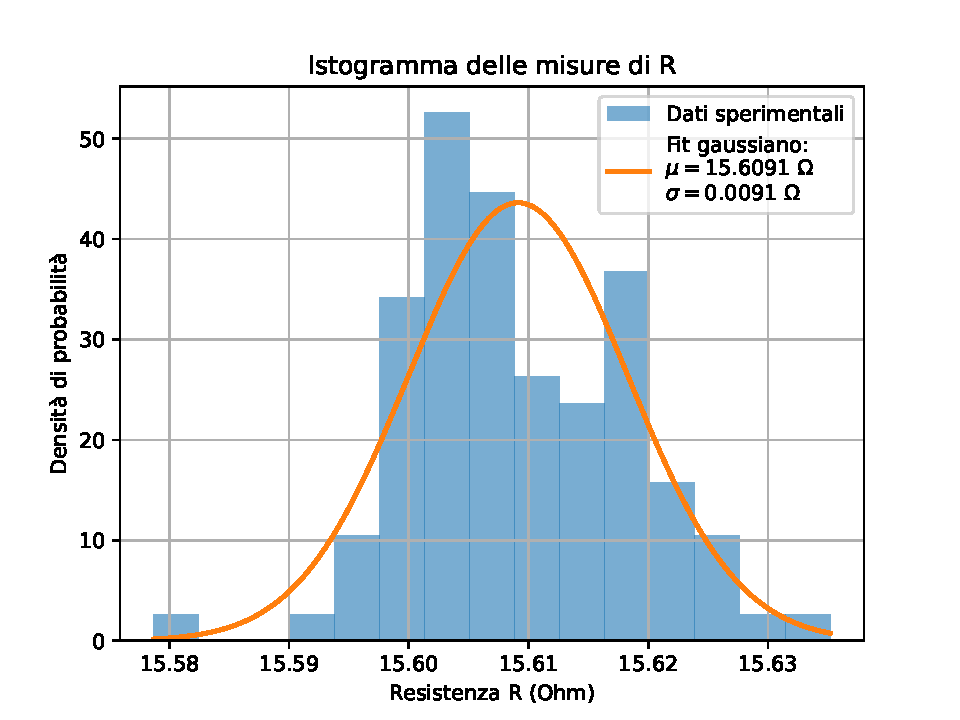
\includegraphics[width=0.75\linewidth]{figures/istogramma_R_fit_gaussiano.pdf}
    \caption{Istogramma normalizzato e fit gaussiano delle misure di resistenza. La $\sigma$ riportata è campionaria.}
    \label{fig:placeholder}
\end{figure}

\begin{figure}[H]
    \centering
    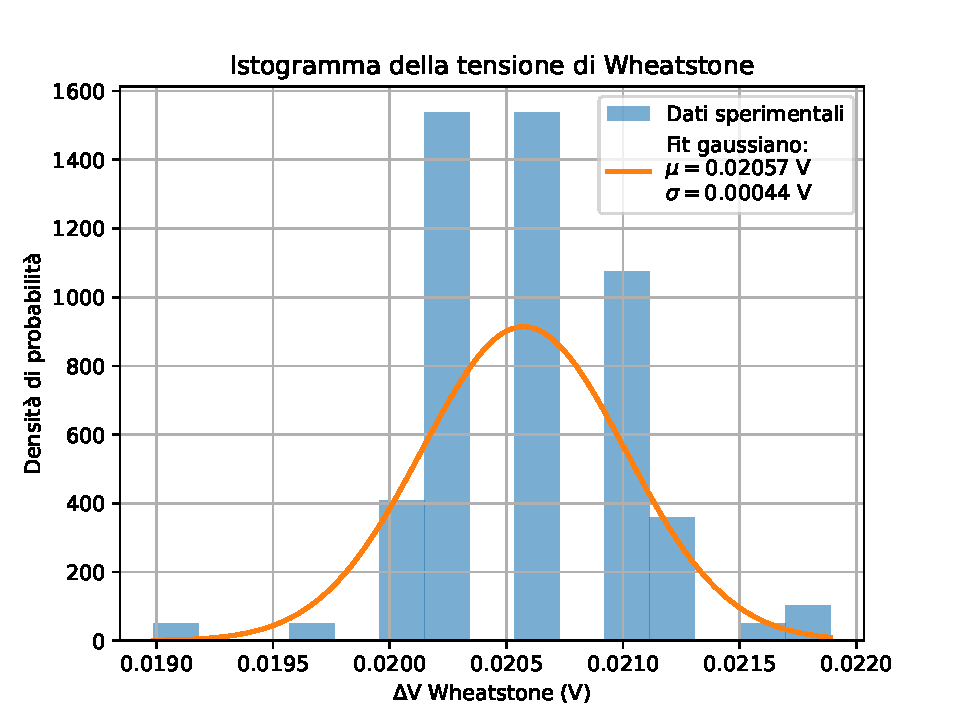
\includegraphics[width=0.75\linewidth]{figures/istogramma_dV_fit_gaussiano.pdf}
    \caption{Istogramma normalizzato e fit gaussiano delle misure di $V_w$. La $\sigma$ riportata è campionaria.}
    \label{fig:placeholder}
\end{figure}

Nelle immagini sopra (Figure 2 e 3) sono riportati i grafici associati al fit gaussiano per di resistenza e tensione della resistenza da $15\Omega$.

La sensibilità del ponte diminuisce con l'aumentare della resistenza (Tabella 3), dunque, l'incertezza relativa tende a diminuire all’aumentare del valore misurato perché la misura assoluta $\Delta R$ rimane approssimativamente costante, mentre il denominatore R cresce.
Dall'ultima riga della tabella possiamo osservare che, variando la portata di $V_w$ e $V_0$, le incertezze rimangono uguali. Ciò probabilmente accade perchè la dispersione dei dati è dominata dal rumore elettronico di fondo e dalle fluttuazioni del ponte.

Le misure di resistenza ricavate mediante il ponte di Wheatstone (Tabella 3) risultano compatibili, entro le incertezze sperimentali e la tolleranza dei valori di riferimento, con i valori nominali attesi.





\end{document}